%----------------------------------------------------------------
%
%  File    :  chapter3.tex
%
%  Authors : Michael Fuska, FH Campus Wien, Austria
% 
%  Created : 13 Feb 2016
%
%  Changed :  
% 
%----------------------------------------------------------------


\chapter{Jailbreak}
\label{ch:JB}

% ------------- JB Allgemein --------------------
\section{Allgemein}
\label{sec:JBAllgemein}

Ein Jailbreak ermöglicht es dem User, die von Apple
vorgesehen Sicherheitsvorkehrung zu umgehen 
Der User erhält durch einen Jailbreak \glqq Zugriff\grqq{} auf das
Betriebsystem und die \glqq Root Zugriffsrechte \grqq{} des Betriebssystem.
Dadurch hat der User die Möglichkeit Applikationen zu installieren,
die nicht von Apple signiert worden sind. 
Mit einem Jailbreak steht dem User, zwei weitere \glqq Application Stores
\grqq{} zur Verfügung.

\begin{description}
\item[Von Apple nicht autorisierte \glqq Applikation Stores\grqq]~\par
	\begin{enumerate}
	   	\item \textbf{Cydia} \cite{Cydia[1]}
		\item \textbf{TaiG}
	\end{enumerate}
\end{description}

% ------------- Arten JB --------------------
\section{Arten von Jailbreaks}
\label{sec:JBArten}
Abhängig von der Art wie sich das iOS Device nach einem Jailbreak verhält, wenn
es rebooted wird, unterscheidet man die Arten von Jailbreaks. 

% ------------- Tethered Jailbreak--------------------
\subsection{Tethered Jailbreak}
\label{sec:JBTethered}
Bei einem \glqq tethered Jailbreak\grqq{} startet das iOS Device nicht nach
einem Reboot. Das iOS Device befindet sich nach einem Reboot im DFU Mode.
Damit das iOS Device wieder gebootet werden kann, muss dieses an einen PC
angeschlossen werden und mithilfe des Jailbreaktools neugestartet werden.

\begin{description}
\item[Zwei Beispiele für \glqq Tethered Jailbreaks\grqq{} sind]~\par
	\begin{itemize}
        \item \textbf{redsn0w}
        \item \textbf{Blackra1n}
    \end{itemize}
\end{description} 

% ------------- Semi Tethered Jailbreak--------------------
\subsection{Semi Tethered Jailbreak}
\label{sec:JBSemiTethered}

Bei einem \glqq Semi Tethered Jailbreak\grqq{} ist es möglich das iOS Device
zu rebooten. Das System startet nicht in den DFU Mode, sondern es ist
mit Einschränkung funktionsfähig. Safari, Mail, Cydia und alle Apps die über
Cydia installiert wurden funktionieren nicht. Das ausführen einer schon
installierten App ermöglicht es dem User, das iOS in einen normalen Zustand zu
bringen. Danach ist das iOS Device vollständig funktionsfähig.

\begin{description}
\item[Ein Beispiel für einen \glqq Semi Tethered Jailbreak\grqq{} ist]~\par
	\begin{itemize}
        \item \textbf{SemiTether package}
    \end{itemize}
\end{description} 

% ------------- UnTethered Jailbreak--------------------
\subsection{Untethered Jailbreak}
\label{sec:JBUntethered}

Bei einem \glqq untethered Jailbreak\grqq{} startet das iOS Device nach einem
Reboot ohne weitere Hilfsmittel.  
\begin{description}
\item[Einige Beispiele für \glqq untethered Jailbreaks\grqq{} sind]~\par
	\begin{multicols}{2}
	\begin{itemize}
        \item \textbf{Absinthe}
        \item \textbf{evasi0n7}
        \item \textbf{Pangu}
        \item \textbf{Pangu8}
        \item \textbf{Pangu9}
        \item \textbf{TaiG}
    \end{itemize}
    \end{multicols}
\end{description} 

% ------------- Semi Untethered Jailbreak--------------------
% \subsection{Semi Untethered Jailbreak}
% \label{sec:JBSemiUntethered}

% ------------- Jailbreak History --------------------
\section{Jailbreak History}
\label{sec:JBHistory}

Im Durchschnitt veröffentlicht Apple sieben iOS Updates pro Jahr. 
\begin{description}
\item[Die Software-Updates dienen dazu]~\par
	\begin{enumerate}
	    \item Die Sicherheitslücken des Betriebssystems zu schließen
	    \item Neue Sicherheitsmechanismen für das Betriebssystem einzuführen
	    \item Neue Sicherheitsarchitekturen für Applikationen bereitzustellen
	\end{enumerate}
\end{description} 
 
Seit der Veröffentlichung der ersten iOS Version im Jahr 2007 wurden insgesamt 74 Softwareupdates von Apple bereitgestellt. Darunter befinden sich neun Major-Updates und 65 Minor-Updates. 

\begin{figure}[!ht]
        \centering
                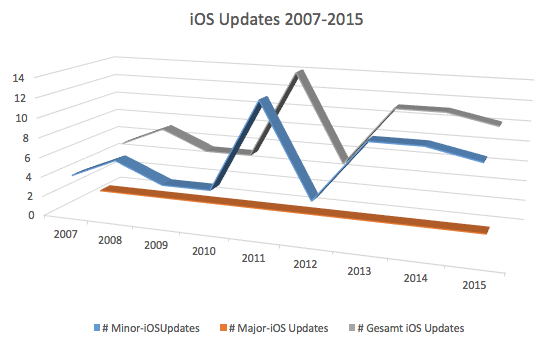
\includegraphics[scale=0.7]{Bilder/iOSUpdates}
        \caption{iOS Software Updates\cite{Apple[7]}}
        	\label{fig:iOS Software Updates}
\end{figure}
% ------ Hard newpage -------

\newpage
Die „Jailbreak-Community“ benötigt im Durchschnitt 36 Tage, um eine neue iOS Version zu „jailbreaken“. Die „Bugs“, die ein Jailbreak ausnützt, sind meistens in mehreren iOS Versionen vorhanden. Nicht alle „Bugs“ werden von Apple geschlossen, es gibt Jailbreaks, die mehrere Jahre funktionieren. Dies gilt vor allem für ältere iOS Versionen und iOS Devices.

\begin{figure}[!ht]
        \centering
                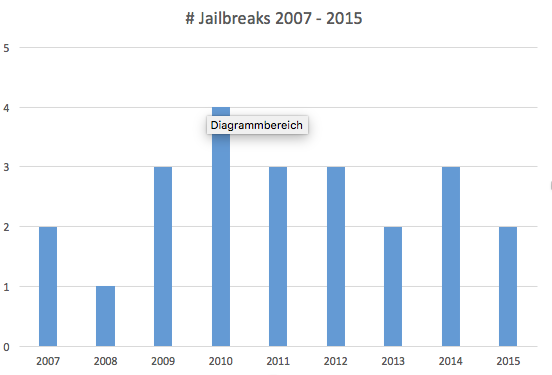
\includegraphics[scale=0.7]{Bilder/AnzahlJB}
        \caption{Anzahl iOS Jailbreak 2007 - 2015}
        	\label{fig:iOS Jailbreak}
\end{figure}


% ------------- Aufbau Jailbreak 9.x --------------------
\section{Aufbau Jailbreak iOS 9.x}
\label{sec:JBAufbau}

\cite{TaiG[1]}
\cite{TaiG[2]}
\cite{TaiG[3]}

% ------------- Jailbreak Step 1 --------------------
\subsection{Breaking out of the sandbox}
\label{sec:JBStep1}

% ------------- Jailbreak Step 2 --------------------
\subsection{Obtaining arbitrary (unsigned) code execution}
\label{sec:JBStep2}

% ------------- Jailbreak Step 3 --------------------
\subsection{Obtaining root}
\label{sec:JBStep3}

% ------------- Jailbreak Step 4 --------------------
\subsection{Patching the Kernel}
\label{sec:JBStep4}
